We next consider a complex entire-muscle model involving motoneurons, sarcomeres and spindles.
The motoneurons and sarcomeres are used to model a \e{motorunit}, which is associated with a specific \e{fibre type} $\tau\in[0,1]$.
Here, $\tau=0$/$\tau=1$ corresponds to slow/fast twitch fibres, respectively.
We choose $\mups\in \N$ different motorunits in a ``motorunit-pool'', specified by $\tau_k,k=1\ldots\mups$.

\subsection{Motoneuron}
The motoneuron model consists of $6$ degrees of freedom and reads as
\begin{align}
	\vq'(t) &= \fmo(\vq(t),\tau) & \vq(0) &= \vnull,
\end{align}
for any fibre type $\tau$.
We will use $\vq^k(t) \in \R^6$ to indicate the current state of the $k$-th motoneuron (of the $k$-th motorunit).
Of special interest is the second component $q^k_2(t)$, which is the voltage on the motoneuron soma.\fix{tomo?}

\fix{motoneuron model parameter interpolation (coolExp)}

\subsection{Sarcomere}
The sarcomere model describes the force development inside a muscle fibre and is taken from \cite{Shorten2007}.
It has $56$ degrees of freedom and is given by
\begin{align}
	\vr'(t) &= \fsa(\vr(t),\tau) & \vr(0) &= \vr_0(\tau),
\end{align}
for any fibre type $\tau$.
There is a set of $105$ (fibre-type dependent) constants for the model, which we denote by $\csa(\tau)\in\R^{105}$.
We denote by $\vr^k(t)\in\R^{56}$ the state of the $k$-th sarcomere model (of the $k$-th motorunit).

\subsection{Spindle}
The spindle is the muscle component responsible for motoneuron feedback, where the model used is from \cite{Mileusnic2006}.
It has $9$ degrees of freedom and is given by
\begin{align}
	\vs'(t) &= \fsp(\vs(t)) & \vs(0) &= \vnull.
\end{align}
We denote by $\vs^k(t)\in\R^9$ the state of the $k$-th spindle model. In real muscles, the number of spindles is independent from the
number of motorunits, but we use $\mups$ here for simplicity.

\subsection{Model connections}
The overall muscle model is
%
\begin{figure}[!htp]
    \begin{center}%
    \begin{tikzpicture}[auto,%
            block_assign/.style ={rectangle, draw=black, very thick, fill=white,%
            text width=10em, text centered, minimum height=3em, inner sep=6pt},%
            block_big/.style ={rectangle, draw=black, very thick, fill=white,%
            text width=14em, text centered, minimum height=3em, inner sep=6pt},%
            block_dashed/.style ={rectangle, draw=black, very thick, fill=white,%
            text width=10em, text centered, minimum height=3em, inner sep=6pt},%
        ]%
        \tikzstyle{stateEdgePortion} = [black, very thick, -latex', shorten >=1pt];
        \tikzstyle{stateEdge} = [stateEdgePortion];
        \tikzstyle{edgeLabel} = [pos=0.5, text centered];
        \tikzstyle{edgeLabelLow} = [pos=0.25, text centered];
        \tikzstyle{edgeLabelHigh} = [pos=0.25, text centered];
        \tikzstyle{line} = [draw, black, very thick, -latex', shorten >=1pt]];
        \tikzstyle{sline} = [draw, black, very thick];
        \tikzstyle{dline} = [draw, black, dashed, very thick, -latex', shorten >=1pt]];
        \tikzstyle{doublearrow} = [draw, black, very thick, <->, -latex', shorten >=1pt, shorten <=5pt, >=stealth]];
%        \tikzstyle{doubledline} = [draw, black, dashed, very thick, <->, -latex', shorten >=1pt, shorten <=5pt, >=stealth]];
        \node [block_big] (neuro)  {{\bf motoneurons} $\vq^k(t)$\\firing times};%
        \node [block_big, below of=neuro, node distance=30mm] (cell)  {{\bf half-sarcomeres $\vr^k(t)$}\\ action potential, active stress};%
        \node [block_dashed, left of=cell, node distance=80mm] (spindle)  {{\bf spindles $\vs^k(t)$} \\ electrical feedback};%
        \node [block_big, below of=cell, node distance=30mm] (mechanics)  {{\bf 3D continuum mechanics} \\ geometry, deformation};%
        \path [line] (neuro) -- (cell) node[edgeLabel]{$q^k_2(t)$};
        \draw (cell.south) edge[stateEdge] node[edgeLabel]{activation $\alpha(X,t) = \sum\limits_{k=1}^\mups w_k(X) r^k_{53}(t)$} (mechanics.north);
        \path [line] (mechanics) -| (spindle) node[edgeLabelHigh]{$\dla(X_k),\la''(X_k)$};
    	\path [line] ($(neuro.west) + (0,0.3)$) -| ($(spindle.north) + (-0.5,0)$);
    	\path [line] ($(spindle.north) + (0.5,0)$) |- ($(neuro.west) + (0,-0.3)$);
      	\node at (-5.7,-0.7) {$\gamma_{spin}(t)$};
    	\node at (-5.8,0.8) {$freq(q^k_2(t))$};
    \end{tikzpicture}%
    \end{center}%
    \caption{Test}
\end{figure}


\subsubsection{Motoneuron to Sarcomere}
The motoneuron soma signals $q^k_2(t)$ are used to provide activation spikes for the $k$-th sarcomere.
As the sarcomere model merely reacts to high spikes, the motoneuron output is scaled by a nonlinear function $\gamma$ to emphasize high peaks.
Essentially, the small signals are multiplied by a small factor $\beta_m = 0.3$, and the high signals are intensified by $\beta_M = 7$.
The transition from low to high factor is realized by a smooth Gaussian,
where we choose a threshold signal of $q_M = 40$ to pinpoint the signal from which on the $\beta_M$ factor is applied:
\begin{align}
	\gamma(q) &:= \begin{cases}
		\beta_m + e^{-(q-q_M)^2/150}(\beta_M-\beta_m), & 0 < q < q_M\\
		\beta_M & q \geq q_M,
	\end{cases}
\end{align}
Figure \ref{MSLink} illustrates the 
\begin{figure}[!ht]
	\centering
	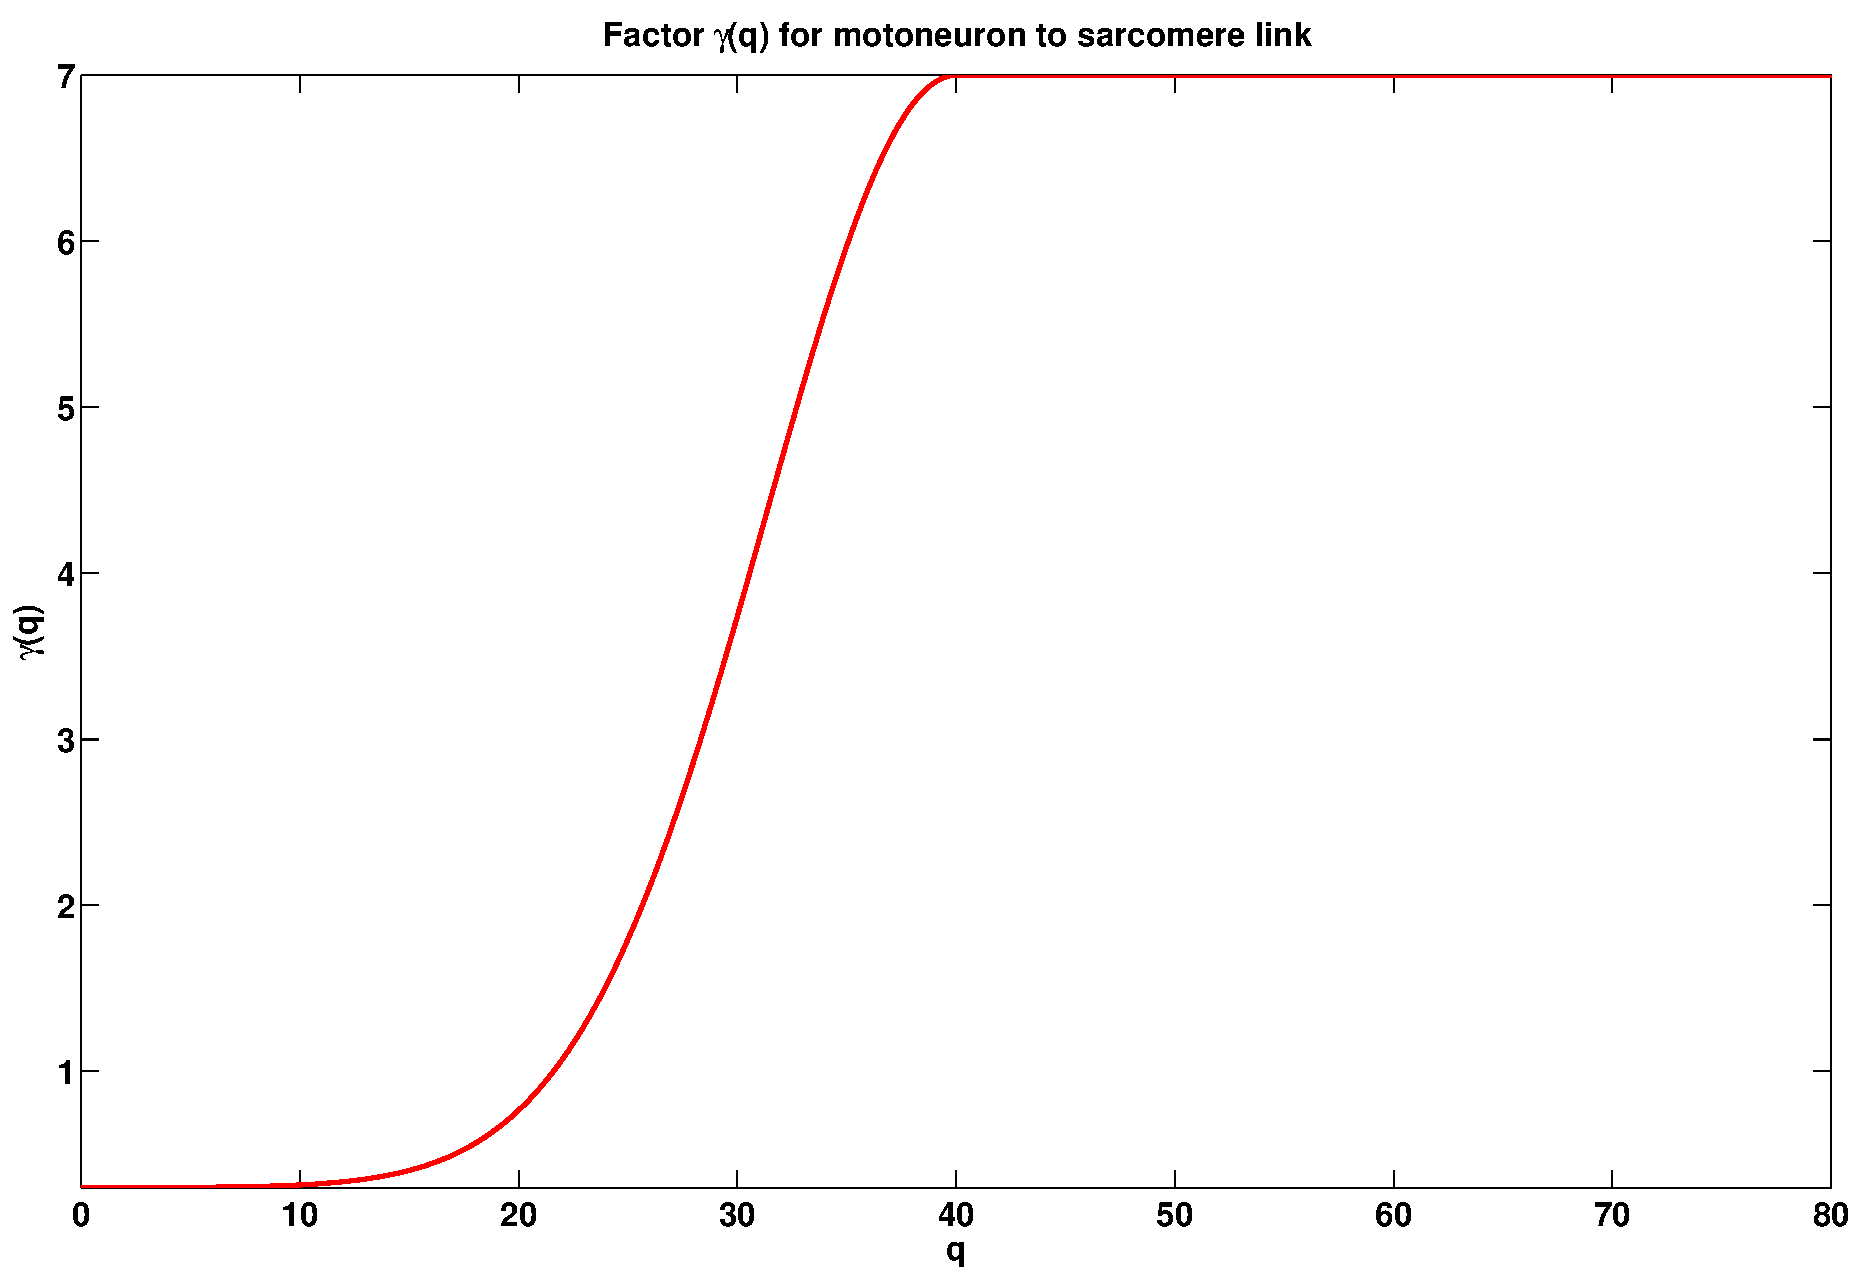
\includegraphics[width=\single]{moto_sarco_link_factor.pdf}
	\caption{Amplification factor for motoneuron signals}
	\label{fig:MSLink}
\end{figure}
Taking into account division by sarcomere model constants, the sarcomere models now read as
\begin{align}
	\vr^k'(t) &= \fsa(\vr^k(t),\tau_k) + \ve_1 \frac{\gamma(q_2^k(t))}{\csa_1(\tau_k)}q_2^k(t),
\end{align}
where $\ve_1 \in \R^{56}$ denotes the first unit vector, i.e. the signal is added to the first component of the sarcomere models.

\subsubsection{Sarcomere to Mechanics}
\subsubsection{Mechanics to Spindle}
\subsubsection{Spindle to Motoneuron}
\subsubsection{Motoneuron to Spindle}
